\documentclass[fleqn,landscape,titlepage,german]{myslides}
%
% Praesentation der Projektgruppe TPML 2.0, 2007
%
% 2007 Christian Fehler
% 2007 Christoph Fehling
% 2007 Benjamin Mies
% 2007 Michael Oeste
%

\usepackage{amssymb}
\usepackage[utf8]{inputenc}
\usepackage{german}
\usepackage{ngerman}

% TP Latex Macros
% tpml
\newcommand{\TPML}{\textsf{\textmd{TPML}}}
\newcommand{\TPMLTWOZERO}{\textsf{\textmd{TPML 2.0}}}

% tp
\newcommand{\TPONE}{Theorie der Programmierung I}
\newcommand{\TPTWO}{Theorie der Programmierung II}

% languages
\newcommand{\LZEROCBN}{$\mathcal{L}_0^{CBN}$}
\newcommand{\LONECBN}{$\mathcal{L}_1^{CBN}$}
\newcommand{\LTWOCBN}{$\mathcal{L}_2^{CBN}$}
\newcommand{\LTWOO}{$\mathcal{L}_2^{O}$}
\newcommand{\LTWOC}{$\mathcal{L}_2^{C}$}

% small step
\newcommand{\smallsteprule}[2]{\begin{array}{@{}c@{}} #1 \\ \hline #2 \end{array}}

% big step
\newcommand{\eval}{\Downarrow}
\newcommand{\bigsteprule}[2]{\begin{array}{@{}c@{}} #1 \\ \hline #2 \end{array}}

% other
\newcommand{\catchword}[1]{\\-\ #1}
\newcommand{\bproduction}{\[\begin{array}{rrlll}}
\newcommand{\eproduction}{\end{array}\]}
\newcommand{\is}{& ::= &}
\newcommand{\al}{\\ & \mid &}

% Einkommentieren, um Handouts zu generieren
%\createhandoutstrue

\begin{document}

\presentation[TPML 2.0] {Christian\ Fehler,\ Christoph\ Fehling,\ Benjamin\ Mies,\ Michael\ Oeste}
                        {TPML 2.0 - Ein interaktives Lernwerkzeug}

\maketitle

\addoverviewitem{Einleitung}
\addoverviewitem{Benutzerfreundlichkeit: Outline, Parser-Autovervollständigung}
\addoverviewitem{Weitere Sprachen: Call by Name, Objekte und Klassen}
\addoverviewitem{\LaTeX-Export}
\addoverviewitem{Neue Beweise: Type Inference, Minimal Typing und Subtyping}
\addoverviewitem{Fazit}

\CenteredGraphics

%%
%% Einleitung
%%
\makeoverviewslide
\myslide{Die Vorlesungen}{
  \begin{itemgroup}{\glqq\TPONE \grqq}
    \item Vermittelt Grundlagen von Programmiersprachen anhand einfacher funktionaler Programmiersprache (orientiert an O'Caml)
    \item Operationelle Semantik anhand von small und big steps
    \item Rekursion
    \item Pflichtveranstaltung für Informatikstudenten
  \end{itemgroup}
}

\myslide{Die Vorlesungen}{
	\begin{itemgroup}{\glqq\TPTWO \grqq}
	 \item Erweiterung um zusätzliche Konzepte:
	 \item Polymorphie
	 \item Typinferenz
	 \item Objekte und Klassen
	 \item bald: Subtyping
	 \item Wahlveranstaltungen im Bereich theoretische Informatik
	\end{itemgroup}
}

\myslide{Motivation I}{
  {\bf Frage:} Warum ein Programm zur \glqq Theorie der Programmierung\grqq?

  \animate{1}{
    \begin{itemgroup}{Gründe}
      \item Erleichterter Zugang zu theoretischen Inhalten
      \item Regelwerk durch \glqq praktisches Arbeiten\grqq\ besser verständlich
      \item \glqq Gefühl\grqq\ für Interpreter und Typsysteme vermitteln
      \item Hilfestellung bei der Prüfungsvorbereitung ($\to$ nicht auf Beispiele aus Übung/Vorlesung beschränken)
      \item Verständnis für Zusammenhang von Programmtext und Ausführung auf einer Maschine
    \end{itemgroup}
  }
}

\myslide{Motivation II}{
  \begin{itemgroup}{Warum nicht O'Caml?}
  % Voller Funktionsumfang von Anfang an Sichtbar
  % Es ist vor allem eine schrittweise, interaktive Beweisführung gewünscht. Diese ist mit O'Caml nicht möglich
  % Weiterhin ist ein Commandozeilentool nicht intuitiv genug. Das Erstellen von GUIs für O'Caml allerdings noch nicht sehr komfortabel.
    \item \glqq Echte Implementierungen\grqq\ ungeeignet
    \item Abläufe nicht sichtbar für den Benutzer
    \item Typfehler von O'Caml schwer verständlich
    \item Semantik nicht zugänglich\\ ($\to$ wird in Byte/native Code kompiliert)
    \item Fehlende formale Spezifikation
  \end{itemgroup}

  \animate{1}{
    {\bf Folgerung:} Spezielles Lernprogramm besser geeignet.
  }
}

\myslide{Die Sprachen I}{
  \begin{itemgroup}{TPML modular/erweiterbar}
  % Genau wie die Vorlesung soll in TPML mit einfachen Sprachen begonnen werden,
  % die Schritt für Schritt erweitert werden.
  % Bei jedem Leistungsstand soll das Tool gleichermaßen einfach bedienbar sein.
    \item Beginn mit  einfachen Sprachen
    \item Inkrementelle Erweiterung
    \item Bis zu imperativen und objekt-orientierten Konzepten
    \item Lernprogramm soll diese Lernkurve wiederspiegeln
  \end{itemgroup}
}

\myslide{Die Sprachen II}{
  \begin{itemgroup}{Die Sprachen im Überblick}
% Liste der verfügbaren Sprachklassen
    \item ${\cal L}_0$ - ungetypter $\lambda$-Kalkül
    \item ${\cal L}_1$ - einfach getypter $\lambda$-Kalkül
    \item ${\cal L}_2$ - ${\cal L}_1$ mit Rekursion
    \item ${\cal L}_3$ - polymorph getypte Sprache mit Listen und Tupeln
    \item ${\cal L}_4$ - imperative Konzepte (Speicher, Schleifen)
  \end{itemgroup}
}

\myslide{Die Sprachen III}
{
% Wo sinnvoll existiert für jede Sprache eine "Untersprache" für diese Erweiterungen
	\begin{itemgroup}{Spracherweiterungen}
	\item{Call-by-Name Semantik}
	\item{Objekte und Klassen}
	\item{Subtyping: Nachweis von Subtyprelationen}
	\end{itemgroup}
}

\myslide{Die Sprachen IV}{
  \begin{itemgroup}{Realisierung}
  % Durch Auswahl der Sprache legt der Benutzer die Komplexität des Tools implizit fest.
  % So ist gewährleistet,dass die Komplexität des Tools mit der Kompetenz des Users wächst. 
    \item Benutzer wählt beim Erstellen neuer Datei eine Sprache
    \item Sprache bestimmt dann Programmverhalten (Typregeln,\\ Semantikregeln, Syntaxhighlighting, \ldots)
	\item Ausgewählte Sprache beeinflusst verfügbare Beweiswerkzeuge
  \end{itemgroup}

}


\myslide{Projektgruppe TPML 2.0.0}
{
  % Bei TPML 1.0 nur die Sprachklasse aswählbar.
  % nicht kompletter Vorlesungsstoff abgedeckt
  % persistenz fehlt
	\begin{itemgroup}{Ausgangspunkt TPML 1.0.0}
	\item Unterstützt ${\cal L}_0$ - ${\cal L}_4$
	\item keine Unterstützung der Spracherweiterungen
	\item große Ausdrücke teilweise unübersichtlich
	\item kein Export / Drucken der geführten Beweise
	\end{itemgroup}
}

%ZIELE

\myslide{Projektgruppe TPML 2.0.0}
{
% Ziel: Tool insbesondere dann sinnvoll wenn der komplette Stoff unterstützt wird
% sonst doch eher frustrierend
  \begin{itemgroup}{Ziel: Abdeckung des Vorlesungsstoffes}
    \item Vollständige Unterstützung von \glqq\TPONE \grqq
	\catchword{Call-by-Name}
	\catchword{Typinferenz}
	\catchword{Objekte}
    \item Erweiterung um die Inhalte von \glqq\TPTWO \grqq
	\catchword{Klassen}
	\catchword{Subtyping}
  \end{itemgroup}
}

\myslide{Projektgruppe TPML 2.0.0}
{
  \begin{itemgroup}{Ziel: Übersichtlichkeit}
	\item Darstellung von Variablenbindungen
	%Visualisierung bei Mouse Over
	%Eine der ersten Sachen, die in der Vorlesung besprochen werden.
	\item intelligenteres Umbrechen von langen Ausdrücken
	%bisher maximal ein Umbruch
	%Variablenbindungen sonst nicht sichbar
	\item Darstellung des Syntaxbaumes
	%Strukturiertere Darstellung von großen Ausdrücken
	%Einfacheres Erkennen der nun zu verwendenden Regel
	%Erkennen wie ein konkreter Ausdruck aus Items der Abstrakten Syntax aufgebaut ist.
  \end{itemgroup}
}

\myslide{Projektgruppe TPML 2.0.0}
{
  \begin{itemgroup}{Ziel: Komfortfunktionen}
	\item Persistenz der geführten Beweise
	\catchword{PDF Export}
	%target: dau, der drucken will was er sieht
	\catchword{\LaTeX\ Export}
	%target: übungsgruppenleiter, klausurerstellung, da ausgabe bearbeitet werden kann
	\item Autovervollständigung von Ausdrücken
	%Erleichtert schreiben von Ausdrücken
	\item Verbesserung der Fehlermeldungen
  \end{itemgroup}
}

\myslide{Projektgruppe TPML 2.0.0}{
	\begin {itemgroup}{Aufgabenverteilung}
    \item Weiterentwicklung der Kernkomponenten - Christian Fehler, Benjamin Mies
    \item Visuelle Darstellung der Beweiswerkzeuge - Michael Oeste
    \item Benutzerinterface und PDF Export - Christoph Fehling
  \end{itemgroup}
}



%%
%% Outline
%%
\makeoverviewslide
\myslide{Outline}
{
  \begin{itemgroup}{Übersicht}
    \item Ausdrücke und Typen können in ihrer Baumansicht betrachtet werden
    \item Schwierige Ausdrucke können so besser verstanden werden
    \item Name der Ausdücke und Typen wird dargestellt
    \item Menge der Ausdrücke und Typen wird dargestellt
    \item Der Index wird ebenfalls eingeblendet
    \item Bindungen von Identifiern können betrachtet werden
    \item Die Outline muss bei neuen Ausdrücken nicht angepasst werden,
          sondern übernimmt diese automatisch
  \end{itemgroup}
}

\myslide{Outline}
{
  \begin{itemgroup}{Einstellungen}
    \item \glqq Hervorheben\grqq: Selektierte Knoten werden in höheren Knoten markiert
    \item \glqq Gebundene\grqq: Gebundene Identifier werden markiert
    \item \glqq Freie\grqq: Frei vorkommende Identifier werden markiert
    \item \glqq Ersetzen\grqq: Selektierte Knoten werden durch \glqq ...\grqq\ ersetzt
    \item \glqq Source Code\grqq: Der zu dem selektierten Knoten passende Source Code
                                  wird im Editor hervorgehoben
    \item \glqq Auto Update\grqq: Die Outline wird bei Änderungen automatisch aktualisiert
  \end{itemgroup}
}

\myslide{Outline}
{
  \begin{center}
    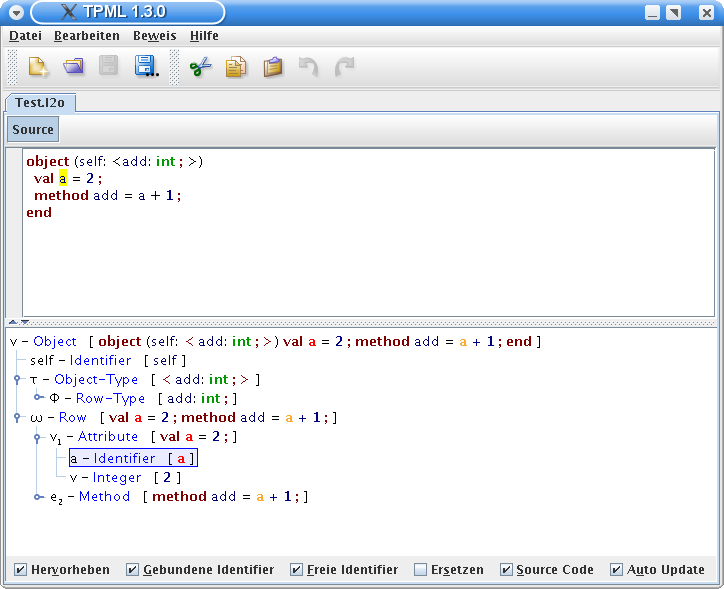
\includegraphics[height=15cm]{images/outline.png}
  \end{center}
}

%%
%% Parser
%%
\myslide{Parser - Autovervollständigung}
{
  \begin{itemgroup}{Übersicht}
    \item Die Parser waren sehr unübersichtlich strukturiert
    \item Pro Ausdruck und Typ wurde ein eigenes \glqq non terminal\grqq eingeführt
    \item Zusätzlich ein eigenes \glqq error non terminal\grqq, welches sich um
          die eingeführte Fehlerbehandlung kümmert
    \item Jedem geparsten Ausdruck wird seine Source Code Position mitgegeben, um
          Fehler anzeigen zu können und, um den Source Code durch die Outline
          markieren zu lassen
    \item Eine automatische Vervollständigung wurde eingeführt, um vom Benutzer
          eingegebene, noch unvollständige Ausdrücke zu vervollständigen
    \item Fehlermeldungen, die mehrere Stellen betreffen, wurden eingeführt
  \end{itemgroup}
}

\myslide{Parser - Autovervollständigung}
{
  Gibt der Anwender \glqq \ExprInfixOperation{+}{1}{\KeyLet\ \ExprIdentifier{x} =}\grqq\ 
  ein, wird der Teil \glqq \KeyLet\ \ExprIdentifier{x} =\grqq\ hervorgehoben und der Tooltip
  verrät dem Anwender, dass er noch den Ausdruck \glqq $e_1$\ \KeyIn\ $e_2$\grqq\ eingeben muss,
  um \glqq{\bf Let}\grqq\ zu vervollständigen. Durch einen Mausklick auf das Symbol wird der
  fehlende Code ergänzt.
  \begin{center}
    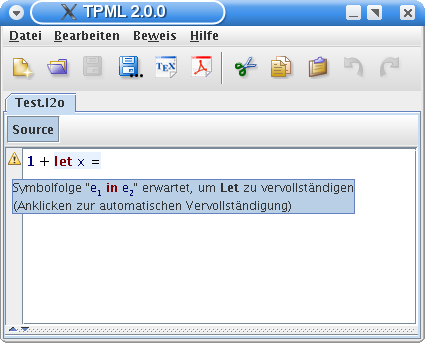
\includegraphics[height=10cm]{images/parser_auto.png}
  \end{center}
}

\myslide{Parser - Fehlermeldungen}
{
  Gibt der Anwender einen Ausdruck ein, der laut Theorie nicht zulässig ist, werden die entsprechenden
  Stellen rot unterstrichen. In diesem Beispiel ist ein Objekt mit Attributen mit dem gleichen Namen
  nicht erlaubt.
  \begin{center}
    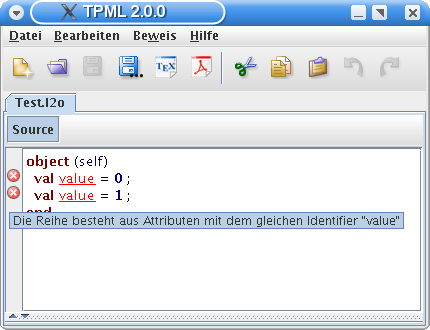
\includegraphics[height=10cm]{images/parser_error.png}
  \end{center}
}

\myslide{Parser - Korrekturen}
{
  Gibt der Anwender einen Ausdruck ein, der laut Theorie nicht zulässig ist, eine Korrektur aber durch
  einfaches Umbenennen möglich ist, wird dies dem Anwender vorgeschlagen. Klickt er auf das blaue Icon,
  werden die entsprechenden Identifier umbenannt.
  \begin{center}
    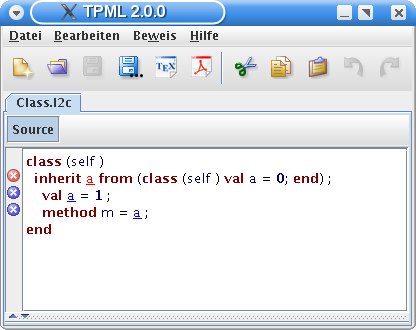
\includegraphics[height=10cm]{images/parser_rename.png}
  \end{center}
}

%%
%% Call by Name
%%
\makeoverviewslide
\myslide{Call by Name}
{
  \begin{itemgroup}{Übersicht}
    \item Sprachen \LZEROCBN, \LONECBN und \LTWOCBN  mit Call by Name Semantik
    \item Ausdrücke werden nicht erst ausgewertet, sondern direkt eingesetzt,
          dadurch kann es zu unterschiedlichen Ergebnissen kommen
    \item Änderung der Small Step Semantik
    \item Änderung der Big Step Semantik
    \item Einführung eigener Dateiendungen
    \item Relevant für die Prüfung \glqq \TPONE \grqq
  \end{itemgroup}
}


\myslide{Call by Name}
{
  {\bf Änderungen:} Small Step Semantik\\[5mm]
  \begin{tabular}{ll}
     \mbox{(BETA-V)}      & nicht vorhanden \\[3mm]
     \mbox{(BETA)}        & $\ExprApplication{\Parenthesis{\ExprLambda{id}{}{e_1}}}{e_2} \to
                                               e_1[e_2/\ExprIdentifier{id}]$ \\[3mm]
     \mbox{(APP-RIGHT)\ } & $\smallsteprule{e \to e'}
                              {v\,e \to v\,e'}$ \ 
                              falls ${v}$ nicht von der Form $\ExprLambda{id}{}{e_0}$ \\[5mm]
     \mbox{(LET-EVAL)\  } & nicht vorhanden \\[3mm]
     \mbox{(LET-EXEC)}    & $\ExprLet{\ExprIdentifier{id}}{}{e_1}{e_2} \to
                                      e_2[e_1/\ExprIdentifier{id}]$ \\[3mm]
  \end{tabular}
}


\myslide{Call by Name}
{
  {\bf Änderungen:} Big Step Semantik\\[5mm]
  \begin{tabular}{ll}
     \mbox{(BETA-V)}      & nicht vorhanden \\[3mm]
     \mbox{(BETA)}        & $\bigsteprule{e_1[e_2/\ExprIdentifier{id}] \eval v}
                              {\ExprApplication{\Parenthesis{\ExprLambda{id}{}{e_1}}}{e_2} \eval v}$ \\[5mm]
     \mbox{(APP)}         & nicht vorhanden \\[3mm]
     \mbox{(APP-LEFT)}    & $\bigsteprule{e_1 \eval v_1 \quad v_1\,e_2 \eval v}
                              {e_1\,e_2 \eval v}$ \\[5mm]
     \mbox{(APP-RIGHT)}   & $\bigsteprule{e_2 \eval v_2 \quad v_1\,v_2 \eval v}
                              {v_1\,e_2 \eval v}$ \ 
                              falls ${v_1}$ nicht von der Form $\ExprLambda{id}{}{e}$ \\[5mm]
     \mbox{(LET)}         & $\bigsteprule{e_2[e_1/\ExprIdentifier{id}] \eval v}
                              {\ExprLet{\ExprIdentifier{id}}{}{e_1}{e_2} \eval v}$ \\[5mm]
  \end{tabular}
}


\myslide{Call by Name}
{
  {\bf Beispiel:} Unterschied von \glqq Call by Name\grqq\ zu \glqq Call by Value\grqq\\[5mm]
  \begin{tabular}{ll}
     Call by Value $\quad$      & $\ExprLet{\ExprIdentifier{x}}{}
                                  {\ExprInfixOperation{/}{\ExprConstant{1}}{\ExprConstant{0}}}
                                  {\ExprConstant{2}} \ \ \to \ \ \ExprExn{divide\_by\_zero}$ \\[3mm]
     Call by Name $\quad$       & $\ExprLet{\ExprIdentifier{x}}{}
                                  {\ExprInfixOperation{/}{\ExprConstant{1}}{\ExprConstant{0}}}
                                  {\ExprConstant{2}} \ \ \to \ \ \ExprConstant{2}$ \\[3mm]
  \end{tabular}
}

%%
%% Objekte
%%
\myslide{Objekte - Übersicht}
{
  \textbf{Aufgabenstellung:}\\[2mm]
  Erweiterung der Sprache \LTWO\ um objektorientierte Konzepte

  \animate{1}
  {
    \begin{itemgroup}{Lösung:}
      \item Einführung einer neuen Sprache \LTWOO
      \item Erweiterung des Scanners und des Parsers
      \item Implementierung neuer Ausdrücke und Typen
      \item Erweiterung aller Beweiswerkzeuge (Small-Step, ...)
      \item Umbau der internen Strukturen, da diese den neuen Anforderungen der
            Theorie nicht genügten (z.B. disjunkte Mengen der verschiedenen Identifier-Gruppen)
    \end{itemgroup}
  }
}

\myslide{Objekte - Interne Struktur}
{
  Identifier werden in Mengen unterteilt: $x \in Var$, $m \in Method$, $a \in Attribute$ 
  und $self \in Self$. Es wird gefordert, dass diese Mengen disjunkt sein müssen,
  dazu müssen die Bindungen zwischen den Identifiern bestimmt werden. Folgendes
  Beispiel ist nicht mehr zulässig:

  \begin{center}
    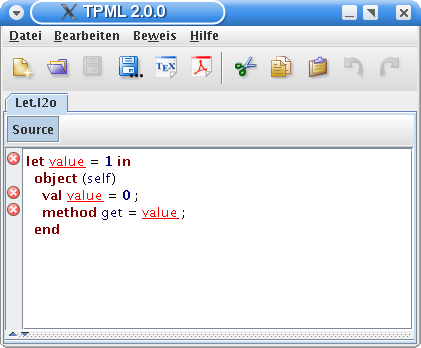
\includegraphics[height=10cm]{images/object_disjunction.png}
  \end{center}
}

\myslide{Objekte - Erweiterung der Produktionen}
{
  \begin{tabular}{lrp{12.0cm}l}
    e      & ::=    & $\Parenthesis{\ExprSend{e}{\ExprIdentifier{m}}}$
                    & \mbox{Methodenaufruf}\\
           & $\mid$ & $\ExprObject{\ExprIdentifier{self}}{\TypeTypeVariable{\tau}}{r}$
                    & \mbox{Objekt}\\
           & $\mid$ & $\ExprDuplication{\ExprIdentifier{$a_1$}\ =\ e_1;\ \ldots\ ; \ExprIdentifier{$a_n$} = e_n}$
                    & \mbox{Duplikation}\\[5mm]

    r      & ::=    & $\ExprRow{\epsilon}$
                    & \mbox{leere Reihe}\\
           & $\mid$ & $\ExprAttribute{\ExprIdentifier{a}}{e}\ r_1$
                    & \mbox{Attribut}\\
           & $\mid$ & $\ExprMethod{\ExprIdentifier{m}}{\TypeTypeVariable{\tau}}{e}\ r_1$
                    & \mbox{Methode}\\[5mm]

    $\tau$ & ::=    & $\TypeRowType{\phi}$
                    & \mbox{Objekttyp}\\[5mm]

    $\phi$ & ::=    & $\TypeRowType{\emptyset}$
                    & \mbox{Leerer Reihentyp}\\
           & $\mid$ & $\TypeRowType{{\ExprIdentifier{m}}\colon\ {\TypeTypeVariable{\tau}}\ ;}\ \phi_1$
                    & \mbox{Methoden-Reihentyp}
  \end{tabular}
}

%%
%% Klassen
%%
\myslide{Klassen - Übersicht}
{
  \begin{itemize}{}
    \item Blablabla ...
  \end{itemize}
}

\myslide{Klassen - Erweiterung der Produktionen}
{
  \begin{tabular}{lrp{12.0cm}l}
    e      & ::=    & $\ExprClass{\ExprIdentifier{self}}{\TypeTypeVariable{\tau}}{b\ }$
                    & \mbox{Klasse}\\
           & $\mid$ & \ExprNew{e}
                    & \mbox{New}\\[5mm]

    b      & ::=    & $\ExprInherit{\ExprIdentifier{$a_1$},\ \ldots\ ,\ExprIdentifier{$a_k$}}{e}{b}$
                    & \mbox{Inherit}\\
           & $\mid$ & r
                    & \mbox{Reihe}\\[5mm]

    $\tau$ & ::=    & $\TypeClassType{\TypeTypeVariable{\tau}}{\TypeTypeVariable{\phi}}$
                    & \mbox{Klassentyp}\\[5mm]

    $\phi$ & ::=    & $\TypeRowType{{\ExprIdentifier{a}}\colon\ {\TypeTypeVariable{\tau}}\ ;}\ \phi_1$
                    & \mbox{Attribut-Reihentyp}
  \end{tabular}

  {\bf Problem:} Methoden- und Attribut-Reihentyp sind durch den Parser nicht unterscheidbar,
                 da dieser nur einen Identifier erkennt.

  \animate{1}
  {
    {\bf Lösung:} Konkrete Syntax:
                  $\TypeRowType{\KeyAttr\ {\ExprIdentifier{a}}\colon\ {\TypeTypeVariable{\tau}}\ ;}
                   \TypeRowType{{\ExprIdentifier{m}}\colon\ {\TypeTypeVariable{\tau}}\ ;}\ \phi_1$
  }
}

%%
%% LaTeX Export
%%
\makeoverviewslide
\myslide{\LaTeX-Export}
{
  \begin{itemgroup}{\LaTeX-Export}
    \item Blablabla ...
  \end{itemgroup}
}

%%
%% Beweise
%%
\makeoverviewslide
\myslide{Neue Beweise: Übersicht}
{
    \begin{itemgroup}{Bisherige Beweisemethoden:}
	\item Smallstepper
	\item Bigstepper
	\item Typechecker
	\end{itemgroup}
    
	\begin{itemgroup}{Neue Beweismethoden:}
	\item Typeinfernce $\to$ Bestimmen eines Typs
	\item Minimal Typing $\to$ Bestimmen eines Typs
	\item SubTyping $\to$ Auflösung von Subtyprelationen
	\end{itemgroup}
  
}

%%
%% Type Inference
%%
\myslide{Outline}
{
  \begin{itemgroup}{Type Inference}
    \item Blablabla ...
  \end{itemgroup}
}

%%
%% Minimal Typing
%%
\myslide{Minimal Typing}
{
  \textbf{Minimal Typing ist ein Beweiswerkzeug, um den Typ für einen Ausdruck zu bestimmen} \\[6mm]
  \begin{itemgroup}{Unterschiede zu Type Checker und Type Inference}
    \item Es gibt keine Typvariablen mehr
      \catchword {Es werden keine Typen mehr geraten}
    \item Es muss ein Typ für die Identifier angegeben werden
      \catchword $\TypeEnvironment{}\ {\vartriangleright}\ {\ExprLet{\ExprIdentifier{x}}{}
         {\ExprInfixOperation{\ExprBinaryOperator{+}}{\ExprConstant{5}}{\ExprConstant{5}}}
         {\ExprInfixOperation{\ExprBinaryOperator{+}}{\ExprIdentifier{x}}{\ExprConstant{2}}}}$
      $\to$ {\color{red}{falsch}}
      \catchword $\TypeEnvironment{}\ {\vartriangleright}\ {\ExprLet{\ExprIdentifier{x}}{\TypeIntegerType}
         {\ExprInfixOperation{\ExprBinaryOperator{+}}{\ExprConstant{5}}{\ExprConstant{5}}}
         {\ExprInfixOperation{\ExprBinaryOperator{+}}{\ExprIdentifier{x}}{\ExprConstant{2}}}}$
      $\to$ {\color{green}{richtig}}
    \item Es wird überprüft ob der angegebene Typ und der berechnete Typ übereinstimmen
      \catchword{Subtyprelation}
    
  \end{itemgroup}
}

%%
%% SubTyping
%%
\myslide{Subtyping}
{
  \begin{itemgroup}{Subtyping}
    \item Blablabla ...
  \end{itemgroup}
}

%%
%% Fazit
%%
\makeoverviewslide
\myslide{Fazit}
{
  \textbf{Projektgruppe \glqq TPML 2.0\grqq}
  \begin{itemgroup}{}
    \item Kleine Projektgruppengröße vorteilhaft
    \item Fast jede Woche eine Besprechung, bei der Fragen zur oder Probleme
          mit der Theorie besprochen werden konnten
    \item Test aller Kernkomponenten vor dem Einsatz in der endgültigen Version
          mit graphischer Oberfläche
    \item Flexible Zielsetzung, inkrementell in kleinen Schritten, trotzdem wurden
          alle angedachten Ziele erreicht
    \item Feedback der Teilnehmer von \glqq TP I\grqq\ bisher durchweg positiv,
          das Feedback der Teilnehmer von \glqq TP II\grqq\ muss noch abgewartet werden
  \end{itemgroup}
}

\end{document}